% !Mode:: "TeX:UTF-8"
% !TEX program  = xelatex
\title{Assignment 3}
% write in preamble: \ctexset{scheme=chinese}


\section{Question 1}
\begin{statebox}{}{question-1}
    Present a study report (3pp+) on American bonds over the past ten years.
\end{statebox}
\subsection{Brief Introduction to U.S. Treasury Bonds}
A United States Treasury security is an IOU from the US Government. It is a government debt instrument issued by the United States Department of the Treasury to finance government spending as an alternative to taxation.
\subsubsection{Some Terms Related With Bonds}
The rate of interest on a bond is referred to as a `coupon rate' and the date when the money is to be paid out is known as the 'maturity' dates. When a savings bond matures, you get the principal amount plus all of the accrued interest. After the maturity date the bond stops earning interest.

Treasury yields are the total amount of money you earn by owning U.S. Treasury bills, notes, or bonds. Generally speaking, the longer the maturity of a Treasury security, the higher the annual yield it will pay, all other factors being equal.

\subsubsection{Analyze the Treasury Yields}
Rates of treasures with different maturity time move up and down somewhat together (They have high correlations).

What moves the yield curve up or down? We can keep in mind that \textbf{the Treasury yield curve reflects the cost of U.S. government debt} and is therefore ultimately a supply-demand phenomenon.

\textbf{If the Fed wants to increase the fed funds rate}, it supplies more short-term securities in open market operations. The increase in the supply of short-term securities restricts the money in circulation since borrowers give money to the Fed. In turn, this decrease in the money supply increases the short-term interest rate because there is less money in circulation (credit) available for borrowers. By increasing the supply of short-term securities, the Fed is yanking up the very left end of the curve, and the nearby short-term yields will snap quickly in lockstep.

When the U.S. government runs a \textbf{deficit}, it borrows money by issuing longer-term Treasury bonds to institutional lenders. The more the government borrows, the more supply of debt it issues. At some point, as the borrowing increases, the U.S. government must increase the interest rate to induce further lending.

If we assume that borrowers of U.S. debt expect a given real return, then \textbf{an increase in expected inflation will increase the nominal interest rate} (the nominal yield = real yield + inflation). Inflation also explains why short-term rates move more rapidly than long-term rates: When the Fed raises short-term rates, long-term rates increase to reflect the expectation of higher future short-term rates; however, this increase is mitigated by lower inflation expectations as higher short-term rates also suggest lower inflation.

\subsubsection{What Factors Create Demand for Treasuries?}
The factors that create demand for Treasuries include \textbf{economic growth, competitive currencies and hedging opportunities}. Just remember: Anything that increases the demand for long-term Treasury bonds puts downward pressure on interest rates (higher demand = higher price = lower yield or interest rates) and less demand for bonds tends to put upward pressure on interest rates.

In environments of falling interest rates, many holders of mortgage-backed securities, for instance, have been hedging their prepayment risk by purchasing long-term Treasuries. These hedging purchases can play a big role in demand, helping to keep rates low, but the concern is that they may contribute to instability.


\subsection{Ten-year Treasury Bonds}
The ten-year treasury bond yield is important because it tends to signal investor confidence. When confidence is high, the ten-year treasury bond's price drops and yields go higher, because investors feel they can find higher returning investments and do not feel they need to play it safe. But when confidence is low, the price goes up as there is more demand for this safe investment and yields fall.

The ten-year treasury is a economic indicator in a sense that its yield tells investors more than the return on investment.  While the historical yield range does not appear wide, any basis point movement is a signal to the market.
\subsubsection{Yield Curve of Ten-year Treasury in Past Ten Years}
\begin{figure}[H]
	\centering
	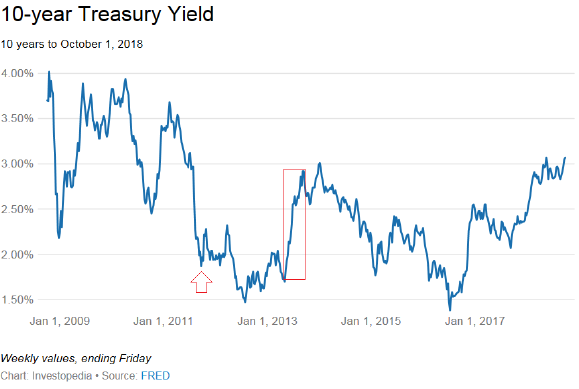
\includegraphics[width=\textwidth]{figures/2019-10-08-yield-curve.png}
	\caption{Yield Curve of 10-year U.S. Treasury Bond}
	\label{F:10yrs-yield-curve}
\end{figure}

\subsubsection{How the Europe Debt Criss Affect the Treasury Yield?}
On June 1, 2012, the benchmark 10-year note yield hit an intra-day low of 1.442 percent, the lowest since the early 1800s.  It was caused by a flight to safety as investors moved their money out of Europe and the stock market (which is due to the Europe debt criss). Investors accepted these low returns just to keep their money safe. They were concerned about the eurozone debt crisis, the fiscal cliff and the outcome of the 2012 Presidential election.

Theoretical explanation: If there is a lot of demand, the bond will go to the highest bidder at a price above the face value. This lowers the yield. The government will only pay back the face value plus the stated interest rate.

In 2013, yields rose 75 percent between May and August alone. Investors sold off Treasurys when the  Federal Reserve announced that it would taper its quantitative easing policy. In December of that year, it began reducing its \$85 billion a month purchases of Treasurys and mortgage-backed securities. The Fed cut back as the global economy improved.

\subsubsection{How the Quantitative Easing Policy Affect the Treasury Yield?}
It is not entirely understood just how much, or even in what direction, the Federal Reserve's quantitative easing, or QE, program affects the bond market. Simple market theory, based on increased demand from homogeneous buyers, should predict that the Fed's purchase programs suppress bond yields below their natural market-clearing level. This assumption also suggests that bond prices are too high, given that yield and price are inverted, to the point of even creating a bubble in the bond market.

Many economists and bond market analysts worry that too much QE pushes bond prices too high due to artificially low interest rates. However, all of the money creation from QE could lead to rising inflation. The chief weapon by the Federal Reserve and other central banks to fight inflation is to raise interest rates. Rising rates could cause massive losses in principal value for bondholders.

\subsubsection{How Trump's election win affect the Treasury yield?}
\begin{quotation}
	Bond investors react to Trump: buy Treasurys (haven!). No wait, sell them (fiscal spending!!). No wait, not that much. \\	--- Chris Whittall (@Chris\_Whittall) November 9, 2016
\end{quotation}

Trump election victory is accelerating a sell-off in long-dated Treasury bonds.

The 10-year Treasury yield on 2016-11-9(Wednesday) surged the most in three years to trade above 2\%, a level not seen since January, on expectations Donald Trump will significantly boost fiscal spending, adding to the country’s debt burden. Analysts also said expectations that Trump will introduce large tax cuts and a significant increase in public spending, particularly on infrastructure, could lead to bigger deficits.



\section{Question 2}
\begin{statebox}{}{question-2}
    How did the yield curve affect the stock market in the US in the recent two years?
\end{statebox}

\begin{quotation}
    The yield curve defines the relationship between interest rates and their maturities. Usually interest rates increase with maturity, reflecting the added return required to compensate for increased risk or inconvenience. 
\end{quotation}
\begin{figure}[H]
	\centering
	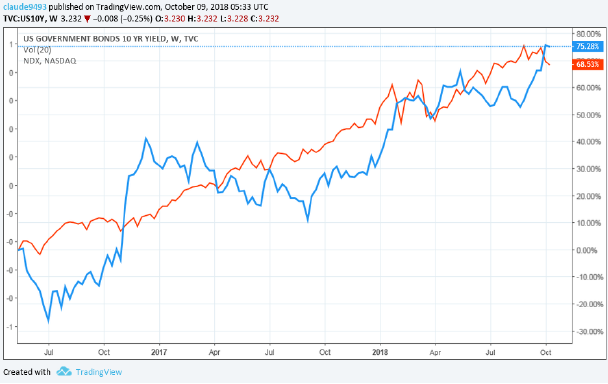
\includegraphics[width=\textwidth]{figures/2019-10-08-US10Y-NASDAQ.png}
	\caption{US10Y and NASDAQ}
	\label{F:us10yvs-nasdaq-2yrs}
\end{figure}
I got the figure of US ten-year treasure yield curve and NASDAQ100 from TradingView.com, the plot is from two years ago. From the figure we can see that \emph{the increase or decrease of yield curve push the NASDAQ100 move in same direction, with much smaller extent}. And I found some view from some professional financial expert:
	
The connection to the stock market is considerably less firm, but ``generally speaking, stocks do better with a moderately positive or fairly steep yield curve,'' relative to the long-term average of 200 basis points, says Sam Burns, research analyst at Ned Davis. The correlation is stronger, Burns says, when one looks at growth and value stocks separately. Over time, he says, an investor would have done well to buy growth stocks when the yield curve became flat (crossing under 200 basis points) and value stocks when the curve became steep (crossing over 200 basis points). 
	
Burns says it stands to reason that a steep yield curve is a signal to buy small-caps. ``Small-caps tend to do better right at the end of a recession at the start of a new bull market, and underperform in the latter part of the cycle,'' he says. ``To the extent that the yield curve goes along with the economic cycle, coming out of recession in the initial leg of an expansion, the steeper yield curve would probably benefit small-caps, while late in the cycle with a flat curve, small-caps don't do as well.''



% \bibliography{ref}
